\documentclass[conference]{IEEEtran}

% Packages
\usepackage{cite}
\usepackage{amsmath,amssymb,amsfonts}
\usepackage{graphicx}
\usepackage{textcomp}
\usepackage{xcolor}
\usepackage{booktabs}
\usepackage{hyperref}
\usepackage{balance}
\usepackage{tikz}
\usetikzlibrary{shapes.geometric, arrows.meta, positioning, fit, backgrounds}
\usepackage{listings}
\lstset{
    language=Python,
    basicstyle=\footnotesize\ttfamily,
    keywordstyle=\color{blue},
    commentstyle=\color{gray},
    numbers=none,
    frame=single,
    breaklines=true,
    captionpos=b
}

\begin{document}

\title{DRIVE: Bridging Theory and Practice in Autonomous Vehicle Education}

\author{
\IEEEauthorblockN{Mohammadparsa Ghasemi, Behnam Bahr, and Viviane Seyranian}
\IEEEauthorblockA{California State Polytechnic University, Pomona\\
Pomona, CA, USA}
}

\maketitle

%==============================================================================
\begin{abstract}
The autonomous vehicle industry's rapid expansion has created unprecedented demand for engineers who can integrate sensing, computation, and actuation into safety-critical cyber-physical systems. Yet most academic programs struggle to provide authentic hands-on experience: simulators abstract away real-world complexity, competition platforms are prohibitively expensive and closed, and small-scale vehicles fail to capture the engineering challenges of full-scale systems. This paper presents DRIVE (Development Research Infrastructure for Vehicle Education), an open-architecture autonomous vehicle research platform developed by converting a 400-pound utility terrain vehicle into a fully instrumented drive-by-wire testbed. Central to the platform is a custom-designed distributed control network built on CAN bus architecture, where students designed the communication protocol, implemented real-time embedded firmware on Teensy microcontrollers, and developed multi-layer safety systems including hardware watchdogs, emergency stops, and fail-safe behaviors. The sensor suite---comprising RTK-GPS with centimeter-level positioning, 3D LIDAR, and vision systems---feeds a modular perception pipeline implementing probabilistic occupancy mapping, costmap generation, and camera-based scene understanding. The platform has served as a testbed for multiple motion planning and control strategies, from graph-based global routing to reactive local planners to geometric path followers, enabling comparative algorithm studies impossible on single-purpose platforms. Unlike commercial research vehicles, every layer of DRIVE---from low-level actuator firmware to high-level planning algorithms---is accessible, documented, and modifiable, transforming the vehicle itself into curriculum. We offer DRIVE as a replicable model for institutions seeking to establish meaningful autonomous vehicle education.
\end{abstract}

\begin{IEEEkeywords}
autonomous vehicles, engineering education, drive-by-wire, CAN bus, closed-loop control, hands-on learning, cyber-physical systems
\end{IEEEkeywords}

%==============================================================================
\section{Introduction}

The autonomous vehicle industry's rapid growth has created urgent demand for engineers who can integrate sensing, computation, and actuation into safety-critical systems. Yet industry leaders report that graduates, while technically competent in isolated domains, lack systems-level integration experience. A National Academies study found that Ford needs more cyber-physical systems engineers ``than we can get,'' while NASA's Jet Propulsion Laboratory reported that 80\% of new hires require substantial internal development due to gaps in integrated systems competencies \cite{nasem2016}. The World Economic Forum identifies this skills gap as a major barrier to business transformation \cite{wef2025}.

Current approaches to autonomous vehicle education each carry significant limitations. Simulation platforms like CARLA and Gazebo democratize access but abstract away real-world complexity---sensor noise, actuator dynamics, and calibration challenges that define physical systems development \cite{virtuallabs2024}. University competitions such as the SAE AutoDrive Challenge provide authentic experiences but require investments exceeding \$200,000, limit access to competition teams, and often use proprietary systems that obscure learning opportunities \cite{autodrive2019}. Small-scale platforms like F1TENTH and Duckietown offer cost-effective alternatives but sacrifice the engineering challenges of full-scale systems: tire dynamics, braking distances, and the safety-critical mindset that comes from operating a vehicle capable of causing harm \cite{f1tenth2024, duckietown2017}. Commercial research platforms provide full-scale authenticity but at costs exceeding \$150,000, accessible only to well-funded research groups.

This paper presents DRIVE (Development Research Infrastructure for Vehicle Education), an autonomous vehicle platform developed at California State Polytechnic University, Pomona by converting a 400-pound utility terrain vehicle into a complete drive-by-wire research testbed. Unlike commercial solutions or competition vehicles, every layer of DRIVE---from low-level actuator firmware to high-level planning algorithms---is accessible, documented, and designed for curriculum integration.

The platform makes three primary contributions. First, we demonstrate a complete drive-by-wire conversion with custom-designed mechanical mounts and closed-loop control on all actuators (steering, throttle, brake), providing students hands-on experience with electromechanical systems integration. Second, we present a distributed embedded control architecture built on CAN bus, where students designed the communication protocol, implemented real-time firmware, and developed multi-layer safety systems. Third, we describe a modular sensor and software architecture supporting multiple perception and planning algorithms, enabling comparative studies impossible on single-purpose platforms. We offer DRIVE as a replicable model for institutions seeking meaningful autonomous vehicle education at a fraction of commercial costs.

%==============================================================================
\section{Platform Design}

\subsection{Base Vehicle Selection}

The base platform is an electric youth utility terrain vehicle powered by a 48V lithium battery system driving a 1.8~kW motor. The vehicle has a net weight of approximately 350 pounds, a 1.23-meter wheelbase, double A-arm front suspension, and rear hydraulic disc brakes. This platform was selected for several reasons: acquisition cost of approximately \$3,000, electric drivetrain eliminating engine complexity while providing a 48V power bus for instrumentation, inherent safety features including roll cage and electronic speed limiting to 27~mph, physical accessibility for undergraduate students, and sufficient payload capacity (440~lbs) for sensors and computing hardware. Fig.~\ref{fig:vehicle} shows the completed platform with sensors mounted.

\begin{figure}[htbp]
\centering
\includegraphics[width=0.9\columnwidth]{vehicle_photo.jpg}
\caption{The DRIVE platform: a converted electric UTV with LiDAR, RTK-GPS, depth camera, and onboard compute.}
\label{fig:vehicle}
\end{figure}

\subsection{Drive-by-Wire Conversion}

Converting the vehicle to drive-by-wire required designing and fabricating custom electromechanical systems for steering, throttle, and braking---each with encoder feedback enabling true closed-loop control. A key design principle was exposing complexity rather than hiding it: students can trace the complete signal path from a steering command issued by planning software through CAN bus transmission, microcontroller processing, motor driver actuation, and encoder feedback. This transparency enables debugging at any level of the system and supports learning objectives across mechanical, electrical, and software engineering curricula. The conversion process itself became a significant educational experience, requiring students to apply mechanical design, power transmission, and control systems concepts to a real vehicle.

\textbf{Steering.} A stepper motor drives the steering column through a custom-designed mounting bracket fabricated to attach directly to the steering shaft. An encoder mounted on the shaft provides absolute position feedback, enabling closed-loop position control with sub-degree accuracy. The stepper motor was chosen for its holding torque and precise positioning without requiring a gearbox.

\textbf{Throttle.} The original mechanical throttle linkage was replaced with electronic throttle control. A wheel speed encoder provides velocity feedback, enabling closed-loop speed control. The control system accepts velocity setpoints and regulates throttle position to maintain the commanded speed, abstracting low-level throttle management from higher-level autonomy software.

\textbf{Brake.} A linear actuator was integrated with the existing hydraulic brake system, pressing the brake pedal mechanism under electronic control. An encoder on the actuator provides position feedback for closed-loop control. The brake system implements fail-safe behavior: loss of communication signal triggers immediate brake application, ensuring the vehicle stops safely if the control system fails.

Table~\ref{tab:actuators} summarizes the closed-loop configuration for each actuator subsystem.

\begin{table}[htbp]
\caption{Actuator Closed-Loop Configuration}
\label{tab:actuators}
\centering
\begin{tabular}{@{}llll@{}}
\toprule
\textbf{System} & \textbf{Actuator} & \textbf{Feedback} & \textbf{Control} \\
\midrule
Steering & Stepper motor & Shaft encoder & Position \\
Throttle & Electronic & Wheel encoder & Velocity \\
Brake & Linear actuator & Position encoder & Position \\
\bottomrule
\end{tabular}
\end{table}

\subsection{Embedded Control Architecture}

The vehicle's control system is built on a distributed Controller Area Network (CAN) architecture with four Teensy 4.1 microcontroller nodes communicating at 250 kbps. The master node handles command parsing from higher-level software and safety arbitration. Three actuator nodes control steering (CAN ID 0x200), throttle (0x100), and braking (0x300), each running closed-loop control algorithms with encoder feedback. Students designed the entire communication protocol from scratch, defining message formats, implementing real-time firmware, and developing safety features including watchdog timers and fail-safe behaviors.

This architecture provides significant educational value. Unlike commercial platforms where students interact with pre-built APIs, DRIVE exposes the complete embedded systems stack. Students can observe CAN traffic, modify control loop gains, implement new message types, and debug timing issues---experiences directly applicable to automotive and robotics industry positions. Fig.~\ref{fig:can} illustrates the distributed CAN architecture.

\begin{figure}[htbp]
\centering
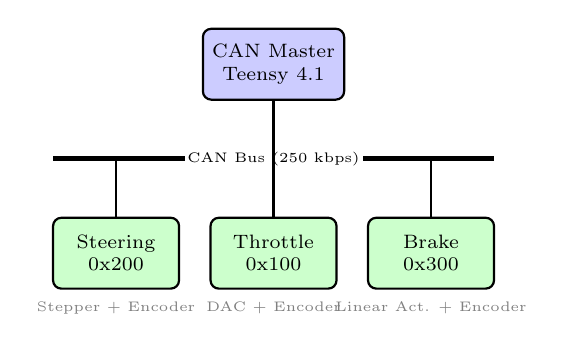
\begin{tikzpicture}[
    node distance=0.6cm,
    box/.style={rectangle, draw, rounded corners=3pt, minimum width=1.6cm, minimum height=0.9cm, align=center, font=\scriptsize, thick},
    masterbox/.style={box, fill=blue!20},
    nodebox/.style={box, fill=green!20},
]
% Master node at top
\node[masterbox] (master) {CAN Master\\Teensy 4.1};

% CAN Bus line
\draw[line width=2pt] (-2.8,-1.2) -- (2.8,-1.2);
\node[font=\tiny, fill=white, inner sep=1pt] at (0,-1.2) {CAN Bus (250 kbps)};

% Vertical drop from master to bus
\draw[thick] (master.south) -- (0,-1.2);

% Actuator nodes
\node[nodebox] (steer) at (-2,-2.4) {Steering\\0x200};
\node[nodebox] (throttle) at (0,-2.4) {Throttle\\0x100};
\node[nodebox] (brake) at (2,-2.4) {Brake\\0x300};

% Connections from bus to nodes
\draw[thick] (-2,-1.2) -- (steer.north);
\draw[thick] (0,-1.2) -- (throttle.north);
\draw[thick] (2,-1.2) -- (brake.north);

% Hardware labels below
\node[font=\tiny, text=gray] at (-2,-3.1) {Stepper + Encoder};
\node[font=\tiny, text=gray] at (0,-3.1) {DAC + Encoder};
\node[font=\tiny, text=gray] at (2,-3.1) {Linear Act. + Encoder};

\end{tikzpicture}
\caption{Distributed CAN bus architecture with four Teensy 4.1 nodes. Each actuator node implements closed-loop control with encoder feedback.}
\label{fig:can}
\end{figure}

\subsection{Network Infrastructure}

A network router serves as the communication backbone, connecting the Jetson Orin AGX (primary compute for GPU-accelerated perception), the CAN master node, and any development laptops via Ethernet (Fig.~\ref{fig:network}). This architecture deliberately avoids tying the platform to a single computer. Students can connect their personal laptops to develop and test code, view sensor data, or manually control the vehicle through a web-based interface. The same backend supports multiple control modalities: joystick control via web UI, voice commands for hands-free operation, and the full autonomous navigation stack.

\begin{figure}[htbp]
\centering
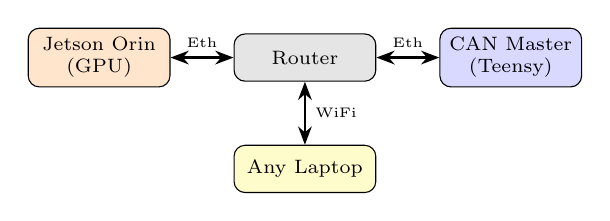
\begin{tikzpicture}[
    node distance=0.8cm,
    box/.style={rectangle, draw, rounded corners, minimum width=1.8cm, minimum height=0.6cm, align=center, font=\scriptsize},
    jetson/.style={box, fill=orange!20},
    router/.style={box, fill=gray!20},
    can/.style={box, fill=blue!15},
    laptop/.style={box, fill=yellow!20},
    >=Stealth
]
% Nodes
\node[jetson] (jetson) {Jetson Orin\\(GPU)};
\node[router, right=0.8cm of jetson] (router) {Router};
\node[can, right=0.8cm of router] (canmaster) {CAN Master\\(Teensy)};
\node[laptop, below=0.8cm of router] (laptop) {Any Laptop};

% Connections
\draw[<->, thick] (jetson) -- (router) node[midway, above, font=\tiny] {Eth};
\draw[<->, thick] (router) -- (canmaster) node[midway, above, font=\tiny] {Eth};
\draw[<->, thick] (router) -- (laptop) node[midway, right, font=\tiny] {WiFi};

\end{tikzpicture}
\caption{Network topology enabling flexible development. Any laptop can connect to develop, test, or control the vehicle.}
\label{fig:network}
\end{figure}

\subsection{Modular Electronics}

Power distribution flows from the vehicle's 48V lithium battery through three DC-DC converters, each feeding its own dedicated fuseblock. Two 48V-to-12V converters provide isolated power domains: one powers the actuator systems (steering motor, throttle controller, brake actuator), while the other powers perception hardware (LiDAR, Jetson compute). This separation ensures that electrical faults in motor drive circuits cannot propagate to sensitive sensor electronics---a deliberate safety decision that students learn to appreciate when debugging intermittent sensor issues.

A dedicated 48V-to-5V converter with its own fuseblock powers the Teensy microcontrollers and encoder electronics, providing a clean logic-level supply isolated from the higher-current 12V domains. Each fuseblock allows individual circuits to be safely isolated during development, enabling students to power only the subsystems they are testing. This modularity reduces risk during debugging sessions and teaches practical lessons about power system design in embedded applications.

The architecture is explicitly designed for expansion---additional CAN nodes, sensors, or actuators can be added without redesigning the power distribution system, supporting the platform's evolution as research needs grow.

%==============================================================================
\section{Sensing \& Software}

The sensor suite comprises industry-grade hardware that exposes students to the same calibration challenges, data formats, and accuracy considerations encountered in professional autonomous vehicle development. Table~\ref{tab:sensors} summarizes the sensor specifications.

\subsection{Sensor Suite}

\begin{table}[htbp]
\caption{Sensor Suite Specifications}
\label{tab:sensors}
\centering
\footnotesize
\begin{tabular}{@{}p{1.2cm}p{1.5cm}p{2.2cm}p{1.8cm}@{}}
\toprule
\textbf{Sensor} & \textbf{Model} & \textbf{Key Specs} & \textbf{Function} \\
\midrule
GPS/IMU & Xsens MTi-680G & RTK: $\pm$5--10~cm$^*$; 9-axis; 100~Hz & Localization \\
LiDAR & Velodyne VLP-16 & 16 layers; 360$^\circ$; 100~m; 10~Hz & Obstacles \\
Depth Cam & Intel RealSense & 640$\times$480 RGB-D; 30~fps & Close-range \\
Compute & Jetson Orin & GPU; Ethernet & Perception \\
\bottomrule
\multicolumn{4}{@{}p{6.7cm}@{}}{\scriptsize $^*$RTK accuracy with correction; degrades to $\pm$2--5~m otherwise}
\end{tabular}
\end{table}

The Xsens MTi-680G provides RTK-capable GNSS/INS positioning with centimeter-level accuracy when RTK correction is available, degrading gracefully to meter-level accuracy otherwise. The sensor outputs position in WGS84 coordinates, velocity and orientation in ENU (East-North-Up) frame at 100~Hz, and reports RTK fix status enabling students to monitor positioning quality in real-time. The General\_RTK filter profile was selected to avoid magnetic interference from the metal vehicle chassis, relying purely on GNSS and inertial fusion for heading estimation. Students examine the \texttt{XsensReceiver} class to understand coordinate frame transformations and thread-safe sensor data management.

The Velodyne VLP-16 provides 360-degree coverage with 16 scanning layers spanning $\pm$15 degrees vertically. At 10~Hz scan rate with 100-meter range and $\pm$2--3~cm accuracy, the sensor generates approximately 300,000 points per second. The UDP-based interface exposes students to network protocols and packet parsing---skills directly applicable to other industrial sensors. Point clouds feed the occupancy grid mapping pipeline for obstacle detection.

Intel RealSense depth cameras provide aligned RGB-D data with factory-calibrated intrinsics, enabling students to focus on perception algorithms rather than calibration procedures. Depth measurements at millimeter resolution support close-range obstacle detection and camera-based scene understanding. The software architecture also supports multi-task neural network perception for lane detection and drivable area segmentation, though the primary perception pipeline relies on LiDAR for obstacle avoidance.

\subsection{Perception Pipeline}

The perception layer provides reference implementations that students can use directly, modify, or replace entirely with their own algorithms. The default occupancy grid uses the log-odds Bayesian framework: each cell maintains a belief that is incrementally updated as observations arrive, with \texttt{log\_odds\_occ} (default 0.4) for occupied cells and Bresenham raycasting marking free space with \texttt{log\_odds\_free} (default $-$0.2). A temporal decay factor causes beliefs to fade toward uncertainty, preventing stale data. The default 40m $\times$ 40m grid at 0.1m resolution suits low-speed navigation, but students can adjust grid dimensions, resolution, and all update parameters to observe effects on detection latency, false positive rates, and convergence behavior.

For motion planning, the probabilistic occupancy grid is transformed into a binary costmap through obstacle inflation. Cells exceeding an occupancy threshold are marked as obstacles, then dilated by the robot radius plus a configurable safety margin using morphological operations. This inflation converts the world representation into configuration space, where a point robot can safely plan without explicit collision geometry. The \texttt{Costmap} class provides efficient single-point collision queries used by the DWA planner.

The perception architecture supports camera-based scene understanding through inverse perspective mapping (IPM) and multi-task neural networks. IPM transforms camera images to bird's-eye view using precomputed homography for real-time performance. While the primary obstacle avoidance relies on LiDAR, the vision pipeline provides lane detection capability for future curriculum modules.

\subsection{Software Architecture}

The software architecture follows a modular sense-plan-control-act pipeline (Fig.~\ref{fig:arch}). In the default configuration, GPS/IMU streams at 100~Hz, LiDAR at 10~Hz, and the control loop at 20~Hz---but all rates are configurable, and students frequently experiment with different timing strategies. This separation allows students to modify any layer independently---implementing a new planner requires only conforming to the waypoint interface, not understanding sensor drivers or actuator protocols. The codebase uses Python with type hints and documentation, prioritizing readability over optimization.

\begin{figure}[htbp]
\centering
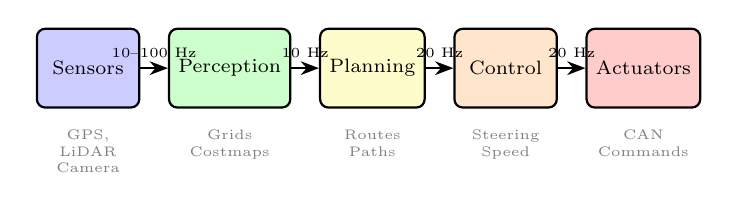
\begin{tikzpicture}[
    node distance=0.3cm,
    stage/.style={rectangle, draw, rounded corners=3pt, minimum width=1.3cm, minimum height=1cm, align=center, font=\scriptsize, thick},
    arrow/.style={->, >=Stealth, thick},
]
% Stages
\node[stage, fill=blue!20] (sensors) {Sensors};
\node[stage, fill=green!20, right=0.35cm of sensors] (perception) {Perception};
\node[stage, fill=yellow!20, right=0.35cm of perception] (planning) {Planning};
\node[stage, fill=orange!20, right=0.35cm of planning] (control) {Control};
\node[stage, fill=red!20, right=0.35cm of control] (actuators) {Actuators};

% Arrows with frequencies
\draw[arrow] (sensors) -- (perception) node[midway, above, font=\tiny] {10--100 Hz};
\draw[arrow] (perception) -- (planning) node[midway, above, font=\tiny] {10 Hz};
\draw[arrow] (planning) -- (control) node[midway, above, font=\tiny] {20 Hz};
\draw[arrow] (control) -- (actuators) node[midway, above, font=\tiny] {20 Hz};

% Labels below (fixed width to prevent overlap)
\node[font=\tiny, text=gray, below=0.15cm of sensors, text width=1.3cm, align=center] {GPS, LiDAR\\Camera};
\node[font=\tiny, text=gray, below=0.15cm of perception, text width=1.3cm, align=center] {Grids\\Costmaps};
\node[font=\tiny, text=gray, below=0.15cm of planning, text width=1.3cm, align=center] {Routes\\Paths};
\node[font=\tiny, text=gray, below=0.15cm of control, text width=1.3cm, align=center] {Steering\\Speed};
\node[font=\tiny, text=gray, below=0.15cm of actuators, text width=1.3cm, align=center] {CAN\\Commands};

\end{tikzpicture}
\caption{Modular software pipeline showing default operating frequencies. All rates are configurable; students can modify any layer independently while interfaces remain stable.}
\label{fig:arch}
\end{figure}

Real-time operation requires careful thread management. The control thread runs in background at 20~Hz, reading sensor state, computing steering commands, and transmitting actuator commands. A \texttt{VehicleState} class provides thread-safe data sharing via lock-protected getters and setters, enabling atomic snapshots that prevent partial reads during control computations. The visualization thread runs in the main process at lower priority, updating displays without blocking control. This architecture teaches practical patterns---producer-consumer synchronization, lock granularity, and non-blocking design---that students encounter in professional robotics software.

The planning layer supports multiple algorithms: global route planning using road network graphs, local reactive planning using the Dynamic Window Approach, and geometric path following using Pure Pursuit with adaptive lookahead. This algorithm diversity enables comparative studies---students can evaluate different approaches on the same physical platform under identical conditions.

\subsection{Accessible API Design}

To lower the barrier to entry while preserving learning depth, DRIVE provides a Python API that abstracts hardware complexity without hiding it. Sensor classes inherit from a common \texttt{SensorInterface} base class providing standardized lifecycle methods (connect, start, stop, disconnect), thread-safe data access, and callback registration. The actuator interface is equally streamlined: controlling the vehicle requires only instantiating \texttt{VehicleActuatorUDP} and calling methods like \texttt{set\_throttle(0.5)} or \texttt{set\_steer\_norm(-0.2)}. Students can begin by treating these as black boxes, then progressively examine the implementation---UDP packet formatting, CAN message construction, encoder feedback---as their understanding grows. This layered design supports the scaffolded learning progression described in Section~IV.

\begin{lstlisting}[float, caption={Simplified API example for vehicle control and sensor access.}, label={lst:api}]
from drive import Vehicle, GPS

# Initialize hardware interfaces
vehicle = Vehicle()
gps = GPS()

# Basic control
vehicle.set_throttle(0.5)   # 50% forward
vehicle.set_steering(-0.3)  # Turn left

# Read sensor data
position = gps.get_position()
heading = gps.get_heading()
\end{lstlisting}

%==============================================================================
\section{Curriculum Integration}

DRIVE was designed explicitly for curriculum integration across multiple engineering disciplines, with its pedagogical approach grounded in established learning theory. To date, fourteen students across three semesters have engaged with the platform, with usage spanning mechanical design projects, embedded systems laboratories, and autonomous systems research.

\subsection{Pedagogical Framework}

The curriculum design follows Kolb's Experiential Learning Cycle \cite{kolb1984}, structuring laboratory activities to progress through concrete experience (hands-on vehicle operation), reflective observation (analyzing system behavior and data logs), abstract conceptualization (connecting observations to control theory and algorithm design), and active experimentation (implementing and testing modifications). This approach addresses findings that hands-on laboratories often fail when students focus solely on active experimentation without structured reflection \cite{abdulwahed2009}.

Learning objectives follow the revised Bloom's Taxonomy \cite{bloom2001}, progressing from foundational knowledge (identifying sensor types, describing algorithm principles) through application (implementing controllers, calibrating sensors) to synthesis (designing integrated autonomous navigation systems). The platform's tangible nature supports constructionist pedagogy, where students construct understanding through building and iterating on physical artifacts---an approach shown effective in robotics education \cite{f1tenth2024}.

\subsection{Learning Modules}

The curriculum comprises six structured modules, each mapping directly to platform software components (Table~\ref{tab:modules}). This structure enables students to examine, modify, and extend production code rather than working with simplified teaching examples.

\begin{table}[htbp]
\caption{Structured Learning Modules}
\label{tab:modules}
\centering
\footnotesize
\begin{tabular}{@{}p{1.5cm}p{3.6cm}p{1.2cm}p{0.6cm}@{}}
\toprule
\textbf{Module} & \textbf{Learning Objectives} & \textbf{Bloom's} & \textbf{Hrs} \\
\midrule
A: Platform \& Safety & Identify architecture; trace sense-plan-act pipeline; operate E-STOP and watchdog & Remember, Understand & 4 \\
B: Sensing & Configure GPS/IMU; interpret RTK status; process LIDAR; calibrate cameras & Apply, Analyze & 6 \\
C: Perception & Implement log-odds occupancy; tune grid parameters; generate costmaps & Apply, Analyze & 8 \\
D: Planning & Compare DWA vs Pure Pursuit; tune cost weights; predict trajectories & Analyze, Evaluate & 8 \\
E: Control & Implement Pure Pursuit; tune PID; validate Ackermann kinematics & Apply, Analyze & 6 \\
F: Integration & Design complete navigation; field validation; document behavior & Create, Evaluate & 12 \\
\bottomrule
\end{tabular}
\end{table}

\subsection{Multidisciplinary Course Integration}

The platform's modular architecture enables targeted engagement across engineering disciplines (Table~\ref{tab:courses}). An Embedded Systems course focuses on CAN bus communication and actuator interfaces (Modules A, B, E), while a Robotics course emphasizes perception and planning algorithms (Modules C, D, F). Senior Design projects leverage the complete platform for capstone experiences.

\begin{table}[htbp]
\caption{Course Integration with Platform Modules}
\label{tab:courses}
\centering
\footnotesize
\begin{tabular}{@{}p{2.6cm}cp{1.3cm}p{1.6cm}@{}}
\toprule
\textbf{Course} & \textbf{Year} & \textbf{Modules} & \textbf{ABET} \\
\midrule
Intro to Engineering & 1 & A & 1 \\
Circuits \& Electronics & 2 & A, B & 1, 6 \\
Embedded Systems & 3 & A, B, E & 1, 6, 7 \\
Control Systems & 3 & D, E & 1, 6 \\
Computer Vision & 3--4 & B, C & 1, 6 \\
Robotics/AI & 4 & C, D, F & 1, 2, 5, 6 \\
Senior Design & 4 & All & 1--7 \\
\bottomrule
\end{tabular}
\end{table}

\subsection{Learning Progression}

Students advance through competency levels via structured activities (Table~\ref{tab:competency}). A student at the Developing level in Control might tune existing PID gains, while a Proficient student implements Pure Pursuit from first principles, and an Advanced student designs adaptive controllers.

\begin{table}[htbp]
\caption{Competency Progression Matrix}
\label{tab:competency}
\centering
\footnotesize
\begin{tabular}{@{}p{1.4cm}p{2.0cm}p{2.0cm}p{2.0cm}@{}}
\toprule
\textbf{Area} & \textbf{Developing} & \textbf{Proficient} & \textbf{Advanced} \\
\midrule
Sensing & Configures sensors; interprets data & Handles noise; fuses sources & Designs calibration \\
Perception & Runs pipelines; visualizes & Tunes parameters; compares & Implements algorithms \\
Planning & Executes planners & Compares; tunes costs & Custom strategies \\
Control & Tunes PID gains & Implements Pure Pursuit & Adaptive control \\
Integration & Connects subsystems & Architects pipeline & Field validation \\
\bottomrule
\end{tabular}
\end{table}

\subsection{Structured Laboratory Activities}

The platform supports six structured laboratories, each designed to develop specific competencies through hands-on engagement with production code (Table~\ref{tab:labs}). Laboratories progress from individual foundational exercises to collaborative integration challenges.

\begin{table*}[htbp]
\caption{Structured Laboratory Activities}
\label{tab:labs}
\centering
\footnotesize
\begin{tabular}{@{}clp{6.2cm}p{2.6cm}cc@{}}
\toprule
\textbf{Lab} & \textbf{Title} & \textbf{Tasks} & \textbf{Key Files} & \textbf{Hrs} & \textbf{ABET} \\
\midrule
1 & Platform Safety & Trace E-STOP signal path; test watchdog timeout; document fail-safes & \texttt{actuators/*.py} & 3 & 1, 2 \\
2 & GPS/IMU Integration & Configure Xsens receiver; log RTK status; transform coordinates & \texttt{xsens\_receiver.py} & 4 & 1, 6 \\
3 & Occupancy Mapping & Tune log-odds parameters; implement raycasting; visualize grids & \texttt{occupancy\_grid.py} & 6 & 1, 6 \\
4 & Planner Comparison & Run DWA and Pure Pursuit; measure and compare metrics & \texttt{dwa.py, pure\_pursuit.py} & 6 & 1, 6 \\
5 & Controller Tuning & Tune Pure Pursuit lookahead; implement PID; validate path & \texttt{pure\_pursuit.py, pid.py} & 5 & 1, 6 \\
6 & System Integration & Integrate modules; conduct field test; prepare report (team) & \texttt{runner.py} & 10 & 1--3, 5, 6 \\
\bottomrule
\end{tabular}
\end{table*}

\textbf{Lab 3: Occupancy Grid Mapping} exemplifies the structured approach. Students run a synthetic obstacle demo, examine log-odds update equations in the \texttt{OccupancyGrid2D} class, modify probability parameters (\texttt{log\_odds\_occ}, \texttt{log\_odds\_free}), measure convergence characteristics, and document parameter sensitivity. Deliverables include a parameter analysis report and modified code with documentation.

\textbf{Lab 6: System Integration} serves as the culminating experience. Teams of 2--3 students integrate perception, planning, and control for autonomous GPS waypoint navigation. Teams define routes using the Navigator module, configure sensor pipelines, select and tune planners, implement safety monitors, conduct field tests with data logging, and present results to peers.

\subsection{ABET Outcome Alignment}

Platform activities map systematically to ABET Student Outcomes (Table~\ref{tab:abet}), demonstrating alignment with accreditation requirements.

\begin{table}[htbp]
\caption{Laboratory Activities Mapped to ABET Outcomes}
\label{tab:abet}
\centering
\footnotesize
\begin{tabular}{@{}lccccccc@{}}
\toprule
\textbf{Laboratory} & \textbf{1} & \textbf{2} & \textbf{3} & \textbf{4} & \textbf{5} & \textbf{6} & \textbf{7} \\
\midrule
Lab 1: Safety & P & P & & S & & & \\
Lab 2: GPS/IMU & P & & & & & P & S \\
Lab 3: Mapping & P & & & & & P & \\
Lab 4: Planning & P & & S & & & P & \\
Lab 5: Control & P & & & & & P & \\
Lab 6: Integration & P & P & P & & P & P & S \\
\bottomrule
\multicolumn{8}{@{}p{7.5cm}@{}}{\scriptsize P = Primary; S = Secondary. 1=Problem-solving, 2=Design, 3=Communication, 4=Ethics, 5=Teamwork, 6=Experimentation, 7=Learning.}
\end{tabular}
\end{table}

%==============================================================================
\section{Assessment \& Outcomes}

\subsection{Skills Developed}

Working with DRIVE develops competencies that employers consistently identify as lacking in new graduates. \textit{Systems thinking} emerges naturally when students observe how a change in one subsystem propagates through others---a modified control gain affects not just actuator response but also planning behavior and safety margins. \textit{Hardware debugging skills} develop through diagnosing real sensor noise, communication dropouts, and mechanical issues that never appear in simulation. \textit{Applied control theory} becomes tangible when students tune PID gains on physical actuators and observe overshoot, oscillation, and steady-state error on a real system. Perhaps most importantly, students develop a \textit{safety-critical mindset}: writing software that controls a 350-pound vehicle changes how one thinks about error handling, testing, and validation.

\subsection{What Hardware Teaches}

Physical systems exhibit behaviors that simulation abstracts away. Encoder readings contain noise and drift over time. Actuators have deadbands where small commands produce no motion, and saturation limits where larger commands produce no additional effect. Mechanical systems exhibit backlash and play. Communication buses occasionally drop messages. These phenomena are not edge cases---they are the defining challenges of real-world autonomous systems. Students who encounter them on DRIVE develop intuition and debugging strategies that transfer directly to industry positions. The physical consequences of software bugs---a vehicle that steers unexpectedly or fails to brake---create learning moments that simulation cannot provide.

\subsection{Assessment Status}

The outcomes described above reflect observations from initial platform deployment rather than formal assessment instruments. As the platform matures and reaches broader student populations, we plan to implement structured pre/post surveys measuring self-reported confidence in systems integration, hardware debugging, and safety-critical development. Quantitative assessment of learning outcomes remains an important direction for future work, as discussed in Section~VII.

%==============================================================================
\section{Discussion}

\subsection{Effective Design Choices}

Several architectural choices proved particularly effective. Router-based networking enabled flexible development---any laptop can connect to the system, eliminating dependence on a single development machine. The fuseblock power distribution system allows safe isolation of subsystems during testing and development. Placing encoders on all actuators enabled true closed-loop control, transforming what could have been open-loop demonstrations into proper feedback control systems. The Teensy 4.1 microcontroller offered an excellent balance of capability, cost, and accessibility, with extensive documentation and an active community.

\subsection{Challenges}

Custom mechanical mounts required access to fabrication equipment (3D printing, machining), which may limit replicability at institutions without maker spaces or machine shops. Initial CAN bus debugging presented a steep learning curve, though this challenge itself became educational. Outdoor testing depends on weather conditions, occasionally limiting platform availability.

\subsection{Cost Analysis}

Table~\ref{tab:cost} presents approximate costs for replicating the platform. The total investment of approximately \$12,000--15,000 is roughly one-tenth the cost of commercial autonomous vehicle research platforms, while providing complete access to all system layers.

\begin{table}[htbp]
\caption{Approximate Platform Costs}
\label{tab:cost}
\centering
\begin{tabular}{@{}lr@{}}
\toprule
\textbf{Component} & \textbf{Cost (USD)} \\
\midrule
Base vehicle & \$3,000 \\
Sensors (LiDAR, GPS, cameras) & \$4,000--6,000 \\
Compute (Jetson Orin AGX) & \$2,000 \\
Electronics (Teensy, actuators, wiring) & \$1,500 \\
Fabrication and miscellaneous & \$1,500 \\
\midrule
\textbf{Total} & \$12,000--15,000 \\
\bottomrule
\end{tabular}
\end{table}

%==============================================================================
\section{Conclusion}

DRIVE demonstrates that meaningful autonomous vehicle education does not require commercial platforms costing hundreds of thousands of dollars or exclusive competition programs. By converting an electric utility vehicle into a complete drive-by-wire research platform with custom CAN architecture, closed-loop control on all actuators, and a modular sensor and software stack, we created an educational tool where every layer---from embedded firmware to planning algorithms---is accessible and modifiable.

The platform addresses a real gap in engineering education: producing graduates who can integrate across mechanical, electrical, and software domains to build safety-critical cyber-physical systems. Students working with DRIVE develop systems thinking, hardware debugging skills, and a safety-critical mindset that simulation-only approaches cannot provide.

Future work includes ROS~2 integration to align with industry-standard middleware, open-source release of firmware and software to support replication at other institutions, expansion to a multi-vehicle fleet for coordination research, and development of formal assessment instruments to measure learning outcomes quantitatively. We offer DRIVE as a replicable model for institutions seeking to establish autonomous vehicle education programs that bridge the gap between academic preparation and industry needs.

%==============================================================================
\section*{Acknowledgment}
This work was supported by the Ganpat and Manju Center for International Collaboration and Innovation at Cal Poly Pomona, established through the generous contribution of Dr. Ganpat Patel and Manju Patel. The DRIVE platform was developed as part of the iCARE-M\&S (Industry 4.0: Career Advancement through Research and Education in Modeling and Simulation) program, which aims to increase the pool of STEM professionals with expertise in autonomous systems. The authors thank the members of the Autonomous Vehicle Laboratory for their contributions to platform development.

%==============================================================================
\begin{thebibliography}{00}

\bibitem{wef2025} World Economic Forum, ``The Future of Jobs Report 2025,'' Geneva, Switzerland, 2025.

\bibitem{nasem2016} National Academies of Sciences, Engineering, and Medicine, ``A 21st Century Cyber-Physical Systems Education,'' Washington, DC: The National Academies Press, 2016.

\bibitem{virtuallabs2024} M. Rahman, S. Ahmed, and K. Patel, ``Effectiveness of Virtual Laboratory in Engineering Education: A Meta-Analysis,'' \textit{PLOS ONE}, vol. 19, no. 3, 2024.

\bibitem{realitygap2017} J. Tobin, R. Fong, A. Ray, J. Schneider, W. Zaremba, and P. Abbeel, ``Domain Randomization for Transferring Deep Neural Networks from Simulation to the Real World,'' in \textit{Proc. IEEE/RSJ Int. Conf. Intell. Robots Syst. (IROS)}, 2017, pp. 23--30.

\bibitem{autodrive2019} J. M. Bastiaan, D. L. Peters, J. R. Pimentel, and M. Zadeh, ``The AutoDrive Challenge: Autonomous Vehicles Education and Training Issues,'' in \textit{Proc. ASEE Annual Conf. Expo.}, Tampa, FL, 2019.

\bibitem{f1tenth2024} J. Betz \textit{et al.}, ``F1TENTH: Enhancing Autonomous Systems Education Through Hands-On Learning and Competition,'' \textit{IEEE Trans. Educ.}, 2024.

\bibitem{duckietown2017} L. Paull \textit{et al.}, ``Duckietown: An Open, Inexpensive and Flexible Platform for Autonomy Education and Research,'' in \textit{Proc. IEEE Int. Conf. Robot. Autom. (ICRA)}, 2017, pp. 1497--1504.

\bibitem{mushr2019} S. S. Srinivasa \textit{et al.}, ``MuSHR: A Low-Cost, Open-Source Robotic Racecar for Education and Research,'' \textit{arXiv preprint arXiv:1908.08031}, 2019.

\bibitem{kolb1984} D. A. Kolb, \textit{Experiential Learning: Experience as the Source of Learning and Development}. Englewood Cliffs, NJ: Prentice-Hall, 1984.

\bibitem{bloom2001} L. W. Anderson and D. R. Krathwohl, Eds., \textit{A Taxonomy for Learning, Teaching, and Assessing: A Revision of Bloom's Taxonomy of Educational Objectives}. New York: Longman, 2001.

\bibitem{abdulwahed2009} M. Abdulwahed and Z. K. Nagy, ``Applying Kolb's experiential learning cycle for laboratory education,'' \textit{J. Eng. Educ.}, vol. 98, no. 3, pp. 283--294, 2009.

\end{thebibliography}

\balance

\end{document}
